% !TeX root = ../../main.tex
\section{Análise de efeitos do lobby}
\label{sec:resultados_efeitos}

Optamos por estimar modelos de contagem via \acrshort{ppml} com \textit{link} logaritmo por três razões principais. Primeiro, as variáveis de interesse (perguntas e reuniões) são contagens, com forte assimetria e alta incidência de zeros no nível MEP–domínio–mês. O \acrshort{ppml} lida naturalmente com zeros sem exigir transformações logarítmicas \textit{ad hoc} que descartam observações. Segundo, o \acrshort{ppml} é consistente sob especificação correta da média condicional mesmo na presença de sobredispersão e heterocedasticidade não especificada, fornecendo erros-padrão robustos quando combinados com \textit{clustering}. Terceiro, a implementação com efeitos fixos de alta dimensão é estável e amplamente utilizada na literatura aplicada (estimador \texttt{fepois} do pacote \texttt{fixest}).

No \acrshort{ppml} com \textit{link} log, a expectativa condicional é \(\mathbb{E}[y\mid X] = \exp(X\beta)\). Assim, para um regressor contínuo \(x_k\) (por exemplo, \textit{meetings} em nível), o coeficiente \(\beta_k\) tem interpretação multiplicativa: um aumento de uma unidade em \(x_k\) está associado a uma variação percentual de \(100\times(\mathrm{e}^{\beta_k}-1)\%\) na média de \(y\), \textit{ceteris paribus}.

A especificação segue o \textit{framework} analítico delineado no capítulo: controlamos por heterogeneidade não observada ao nível do membro e por choques comuns estruturados por partido, país e domínio ao longo do tempo. Concretamente, estimamos modelos com efeitos fixos de membro (\texttt{member\_id}) e efeitos fixos tempo-variantes por país (\texttt{country\_time}), por partido (\texttt{party\_time}) e por domínio (\texttt{domain\_time}). Os erros-padrão são agrupados em \textit{domínio×tempo} e \textit{membro}, capturando correlação serial e choques idiossincráticos nesse nível, conforme implementado nos scripts empíricos.

Essa modelagem garante três propriedades fundamentais para a identificação dos efeitos: (i) permite comparar a evolução da atividade do mesmo \acrshort{mpe} ao longo do tempo, controlando por características não observadas e invariantes como preferências individuais, capital político e produtividade; (ii) elimina a influência de choques ou tendências comuns a todos os \acrshort{mpe}s de um mesmo país ou partido em cada mês, por meio dos efeitos fixos específicos de país$\times$tempo e partido$\times$tempo; e (iii) assegura robustez frente a choques específicos de cada setor ou área temática ao incorporar efeitos fixos de domínio$\times$tempo (\texttt{domain\_time}), isolando variações idiossincráticas desses contextos.

Para testar a Hipótese 1, utilizamos o painel agregado MEP–domínio–mês em amostra combinada (\textit{pooled}) e estimamos PPML com a estrutura de efeitos fixos descrita acima. O coeficiente associado às reuniões (\textit{meetings}) é \textbf{positivo}, indicando que aumentos na intensidade de lobbying estão associados a maior atividade parlamentar em termos de perguntas. Esse resultado é consistente em especificações alternativas, incluindo a versão com termo quadrático para capturar possíveis não linearidades e a inclusão de efeitos fixos \textit{domínio×tempo}, sugerindo robustez do sinal e da magnitude qualitativa do efeito.

Em termos de interpretação, mantidos constantes os efeitos fixos, um incremento marginal em reuniões está associado a um aumento proporcional na média de perguntas dado por \(\mathrm{e}^{\hat{\beta}}-1\). Reportamos os efeitos como variações percentuais estimadas na seção de tabelas de resultados, com intervalos de confiança baseados em erros-padrão agrupados.

\begin{table}[htbp]
\centering
\caption{Resumo dos modelos \acrshort{ppml} para a Hipótese 1}
\label{tab:ppml_h1_both}
\begin{tabularx}{\textwidth}{>{\raggedright\arraybackslash}p{.22\textwidth} >{\raggedright\arraybackslash}X >{\raggedright\arraybackslash}X}
\toprule
  & PPML & PPML (Quad.) \\
\midrule
Reuni\~oes & 0.013*** (0.002) & 0.037*** (0.005) \\
Reuni\~oes$^2$ &  & -0.001*** (0.000) \\
\midrule
Observa\c{c}\~oes & 711,855 & 711,855 \\
Efeitos fixos & \multicolumn{2}{p{.72\textwidth}}{\raggedright pa\'is$\times$tempo; partido$\times$tempo; dom\'inio$\times$tempo} \\
Cluster & \multicolumn{2}{p{.72\textwidth}}{\raggedright dom\'inio$\times$tempo; membro} \\
\bottomrule
\end{tabularx}

\note{A coluna ``DDD PPML'' reporta o modelo principal com efeito linear em \textit{meetings}. A coluna ``DDD PPML (Quadrático)'' adiciona \(\textit{meetings}^2\) para capturar retornos marginais decrescentes. Efeitos fixos: membro; país$\times$tempo; partido$\times$tempo. Erros-padrão agrupados em domínio$\times$tempo e membro.}
\end{table}

\begin{figure}[htbp]
\centering
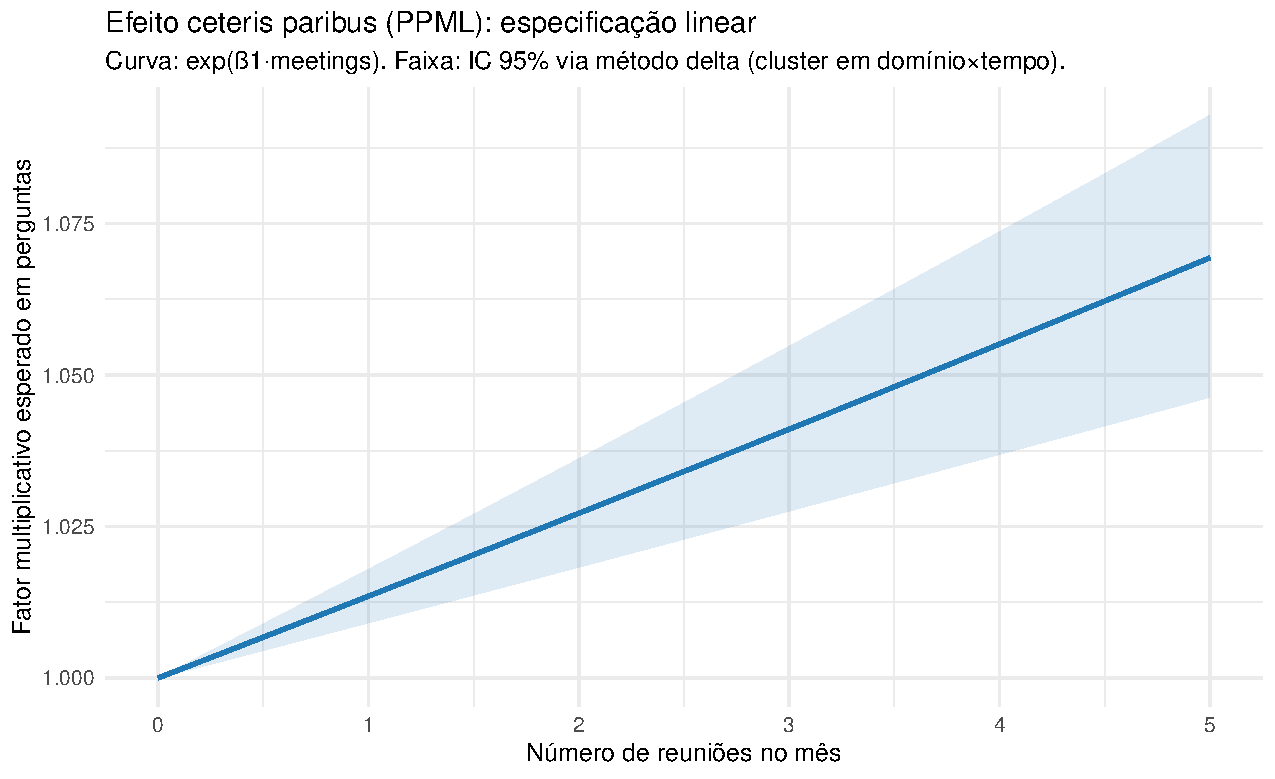
\includegraphics[width=\textwidth]{figures/fig8_effect_linear_ppml.pdf}
\caption{Efeito esperado ceteris paribus: especificação linear (\acrshort{ppml})}
\label{fig:effect_linear_ppml}
\note{A curva apresenta o fator multiplicativo esperado em perguntas como função do número de reuniões no mês, mantendo constantes os efeitos fixos (\(\exp(\hat{\beta}_1\cdot \textit{meetings})\)). A faixa sombreada corresponde ao intervalo de 95\% obtido via método delta com erros-padrão agrupados em domínio×tempo.}
\end{figure}

\begin{figure}[htbp]
\centering
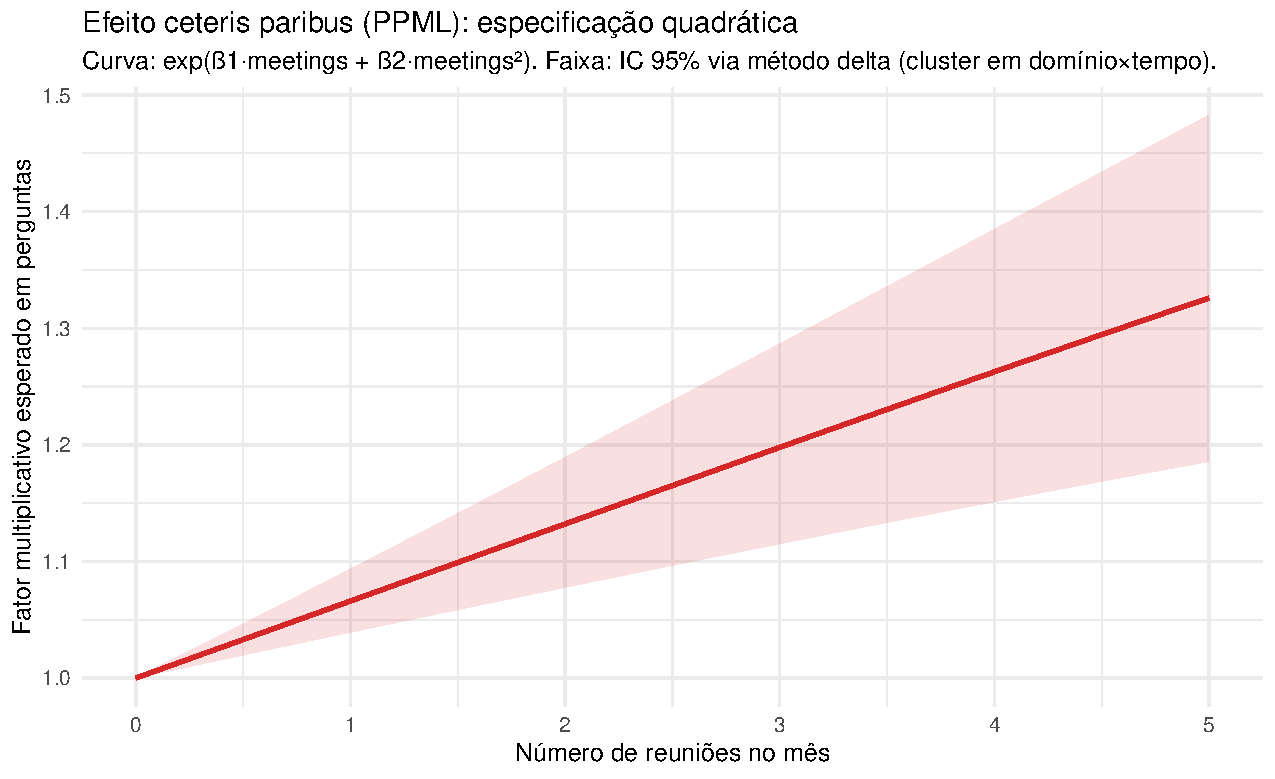
\includegraphics[width=\textwidth]{figures/fig9_effect_quadratic_ppml.pdf}
\caption{Efeito esperado ceteris paribus: especificação quadrática (\acrshort{ppml})}
\label{fig:effect_quadratic_ppml}
\note{A curva apresenta o fator multiplicativo esperado em perguntas como função do número de reuniões, permitindo retornos marginais decrescentes (\(\exp(\hat{\beta}_1\cdot \textit{meetings} + \hat{\beta}_2\cdot \textit{meetings}^2)\)). A faixa sombreada representa o IC de 95\% via método delta com a matriz de variância-covariância agrupada.}
\end{figure}

\autoref{tab:ppml_h1_both} mostra que o coeficiente de \textit{meetings} no modelo \acrshort{ppml} linear é positivo e estatisticamente significativo, evidenciando que aumentos na intensidade de lobbying associam-se a maior número de perguntas, \textit{ceteris paribus}. Na especificação quadrática, o termo linear permanece positivo enquanto o termo quadrático é negativo, indicando retornos marginais decrescentes: o impacto adicional de reuniões sobre perguntas diminui à medida que o volume de reuniões cresce.

Essa interpretação decorre da forma funcional do \acrshort{ppml} (\(\mathbb{E}[y\mid X]=\exp(X\beta)\)). No modelo linear, um acréscimo de uma unidade em \textit{meetings} altera a média condicional de perguntas em \(100\times(\mathrm{e}^{\hat{\beta}_1}-1)\%\). No modelo quadrático, o efeito marginal em log-média é \(\partial\log\mathbb{E}[y\mid X]/\partial\,\textit{meetings}=\hat{\beta}_1+2\hat{\beta}_2\,\textit{meetings}\). Com \(\hat{\beta}_2<0\), esse efeito declina com o nível de \textit{meetings}, isto é, há retornos marginais decrescentes. 

Em particular, a magnitude do termo quadrático é muito inferior ao efeito linear (0,002 vs. 0,066), o que indica retornos marginais decrescentes pequenos na faixa observada. Isso implica que atores com maior disponibilidade de recursos enfrentam pouca perda de eficácia ao intensificar o número de reuniões e, portanto, podem sustentar níveis muito mais altos de lobbying; tal padrão é consistente com a hipótese de que grandes players conseguem alavancar sua capacidade financeira para obter influência relativamente maior, mesmo diante de retornos marginais decrescentes.

As curvas em \autoref{fig:effect_linear_ppml} e \autoref{fig:effect_quadratic_ppml} tornam essa dinâmica visual. A primeira apresenta um efeito multiplicativo crescente de forma monotônica (\(\exp(\hat{\beta}_1\,\allowbreak\textit{meetings})\)), com faixas de incerteza (IC 95\%) obtidas por método delta usando a matriz de variância-covariância com \textit{clustering} em domínio$\times$tempo e membro. A segunda permite curvatura (\(\exp(\hat{\beta}_1\,\allowbreak\textit{meetings}+\hat{\beta}_2\,\allowbreak\textit{meetings}^2)\)) e revela concavidade compatível com saturação de agenda: para níveis altos de \textit{meetings}, o ganho marginal em perguntas é menor. Em ambas as figuras, o eixo horizontal é mantido dentro do suporte observado dos dados para evitar extrapolações.

Do ponto de vista de identificação, os efeitos fixos por membro, país$\times$tempo e partido$\times$tempo controlam heterogeneidade não observada invariável e choques comuns, permitindo comparação \textit{within} do mesmo \acrshort{mpe} ao longo do tempo. A inferência usa erros-padrão agrupados em duas dimensões (domínio$\times$tempo; membro), acomodando dependência serial e seções cruzadas.

Em síntese, os resultados corroboram a Hipótese 1: há associação positiva entre lobbying e atividade de fiscalização medida por perguntas parlamentares, com evidência de retornos marginais decrescentes em níveis mais altos de \textit{meetings}. Essa conclusão é robusta a especificações alternativas consideradas.

A análise desagregada por domínios de políticas públicas revela que o efeito positivo das reuniões sobre a atividade parlamentar é consistente em praticamente todas as áreas temáticas consideradas. Conforme ilustrado na \autoref{fig:effect_linear_ppml_domains}, a estimativa do coeficiente associado a \textit{meetings} permanece positiva em todos os domínios, ainda que a magnitude do efeito varie entre eles. Por exemplo, domínios como "Agricultura" e "Educação" apresentam efeitos mais pronunciados, sugerindo que nesses setores o lobbying pode ser particularmente eficaz em estimular a apresentação de perguntas parlamentares. Já em áreas como "Economia e Comércio" ou "Tecnologia", embora o efeito também seja positivo, sua magnitude é ligeiramente inferior, o que pode refletir diferenças na dinâmica de atuação dos grupos de interesse ou na agenda dos parlamentares nesses temas.

\begin{figure}[htbp]
\centering
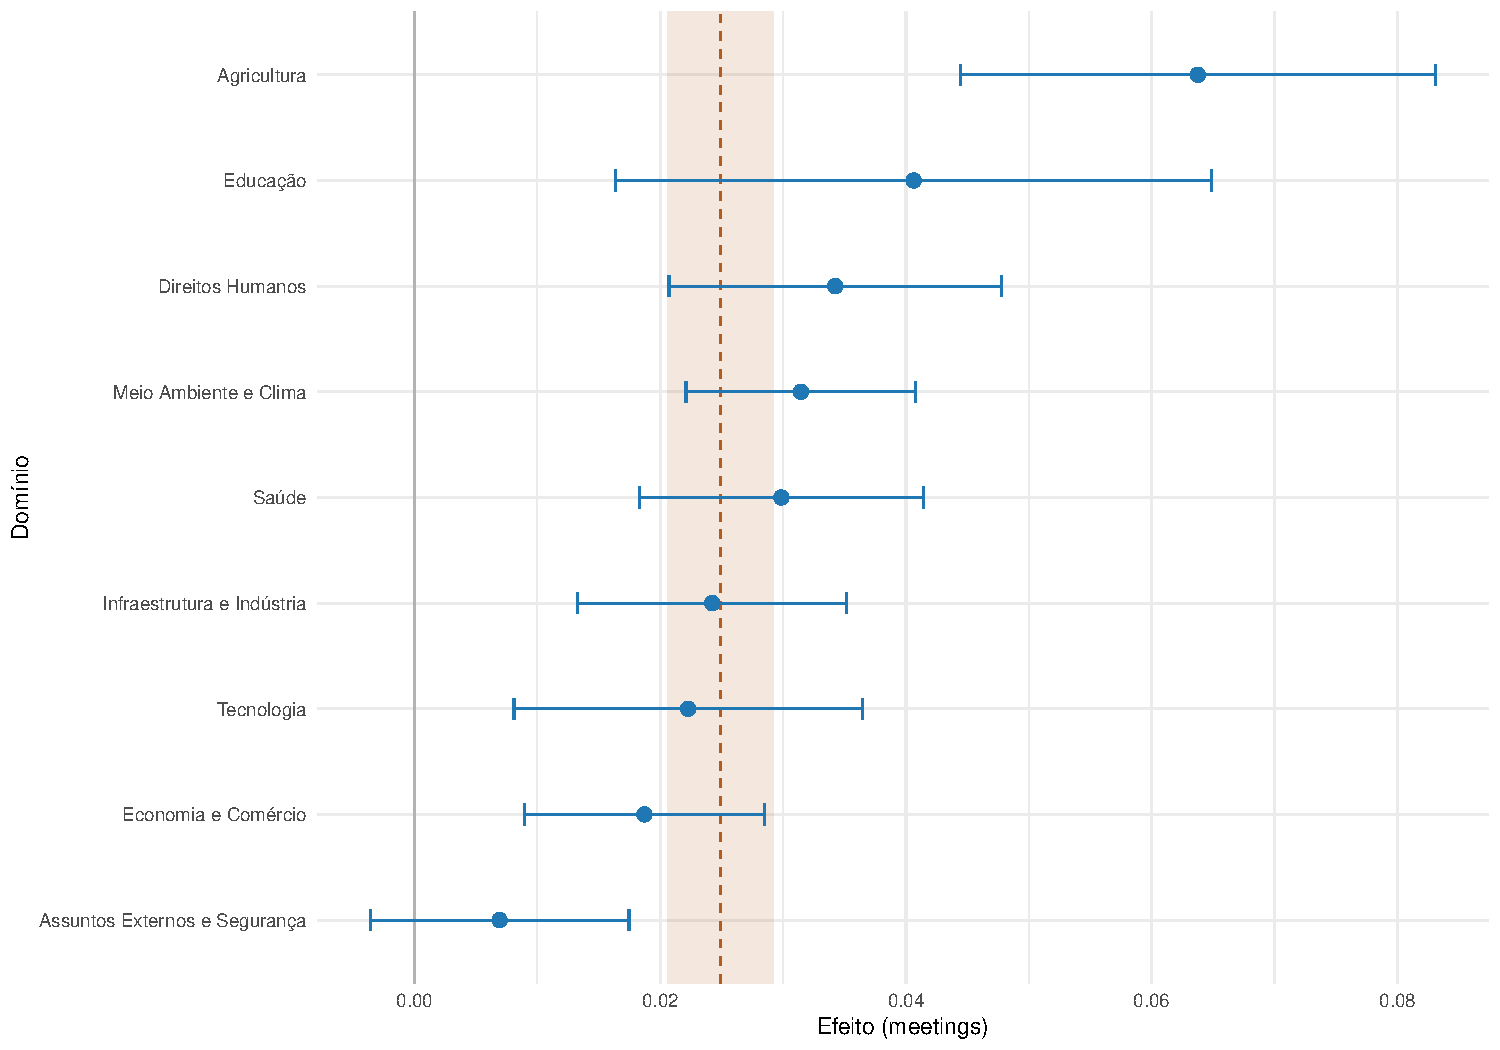
\includegraphics[width=\textwidth]{figures/fig_coeff_domains.pdf}
\caption{Efeito esperado \textit{ceteris paribus}: especificação linear (\acrshort{ppml}) para cada domínio}
\label{fig:effect_linear_ppml_domains}
\note{Cada ponto azul representa a estimativa do coeficiente associado a \textit{meetings} para um domínio específico de políticas públicas, refletindo o efeito marginal esperado de reuniões sobre o número de perguntas parlamentares naquele domínio, mantidos constantes os efeitos fixos. As linhas horizontais correspondem aos intervalos de confiança de 95\% para cada estimativa, indicando a incerteza estatística. A linha tracejada vermelha indica o efeito médio estimado para todos os domínios, servindo como referência para comparação entre áreas temáticas.}
\end{figure}

Além disso, os intervalos de confiança indicam que, apesar de variações na precisão das estimativas entre domínios, o sinal positivo do efeito é robusto e estatisticamente distinto de zero na maioria dos casos. Isso reforça a conclusão de que a associação entre intensidade de lobbying e atividade de fiscalização parlamentar não se restringe a um setor específico, mas se manifesta de forma generalizada no Parlamento Europeu, ainda que com intensidades distintas conforme o contexto temático.

De modo geral, esses resultados sugerem que o impacto do lobbying sobre a produção de perguntas parlamentares é um fenômeno transversal aos diferentes campos de políticas públicas, evidenciando a relevância desse mecanismo de influência em múltiplas agendas legislativas.


% \begin{figure}[htbp]
%     \centering
%     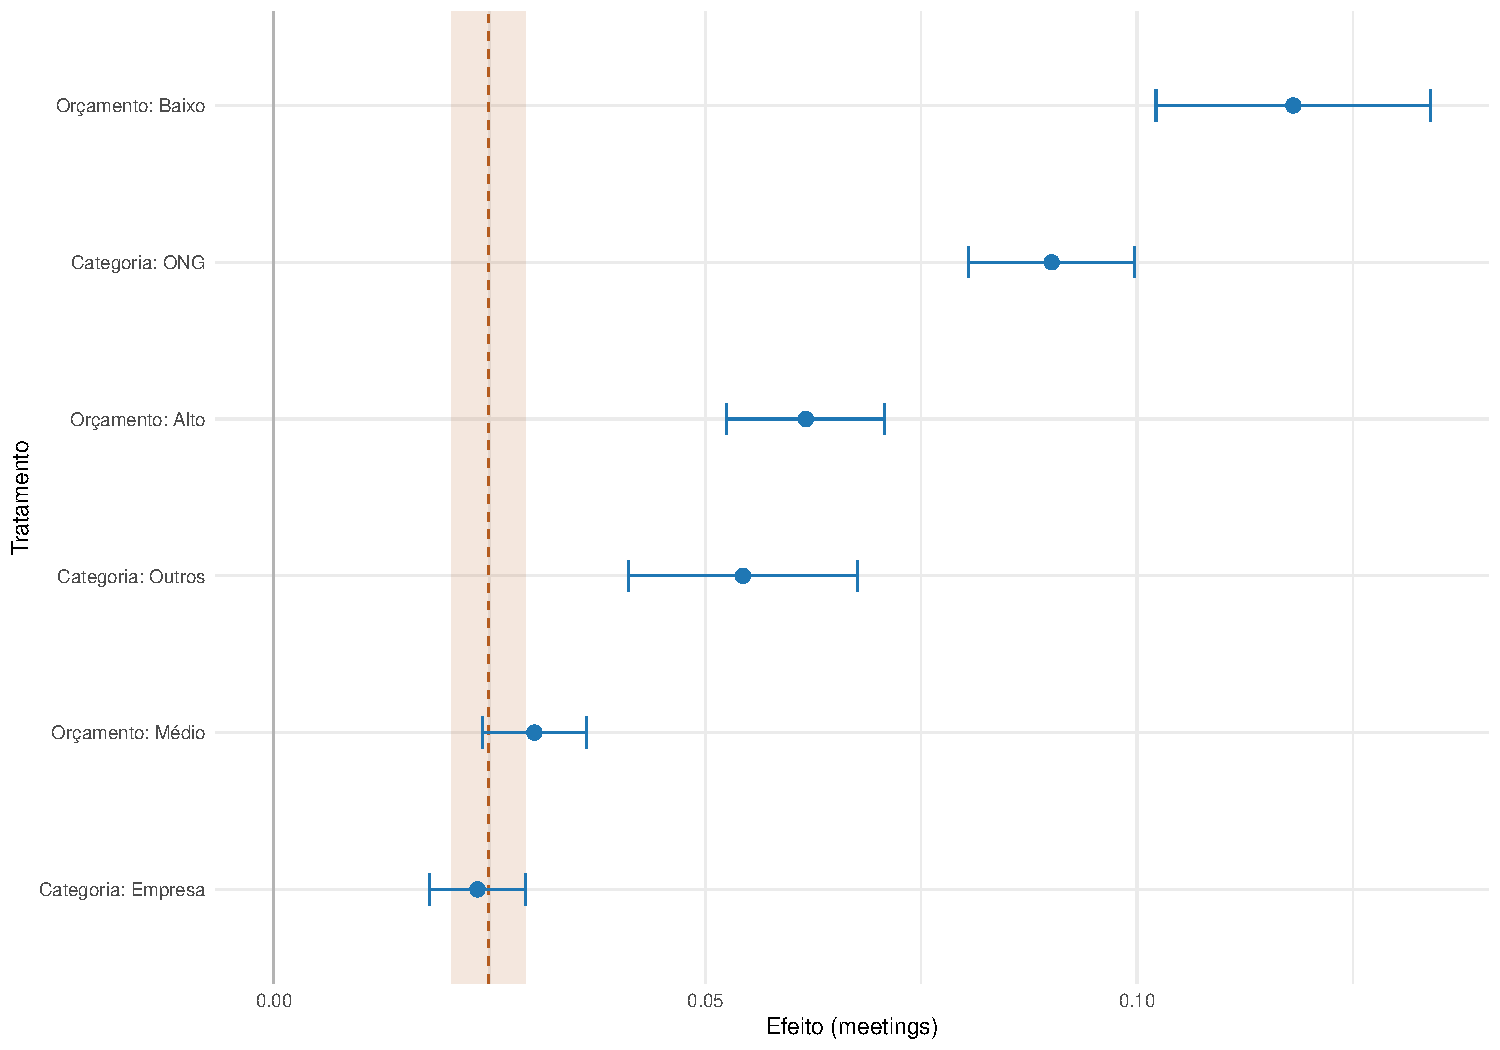
\includegraphics[width=\textwidth]{figures/fig_coeff_treatments_overall.pdf}
%     \caption{Efeito esperado \textit{ceteris paribus}: especificação linear (\acrshort{ppml}) para cada tratamento}
%     \label{fig:effect_linear_ppml_treatments}
%     \note{Cada ponto azul representa a estimativa do coeficiente associado a \textit{meetings} para um tratamento específico, refletindo o efeito marginal esperado de reuniões sobre o número de perguntas parlamentares, mantidos constantes os efeitos fixos. As linhas horizontais correspondem aos intervalos de confiança de 95\% para cada estimativa, indicando a incerteza estatística. A linha tracejada vermelha indica o efeito médio estimado para todos os tratamentos, servindo como referência para comparação entre tratamentos.}
% \end{figure}


\begin{landscape}
\thispagestyle{plain}
\begin{figure}[p]
    \centering
    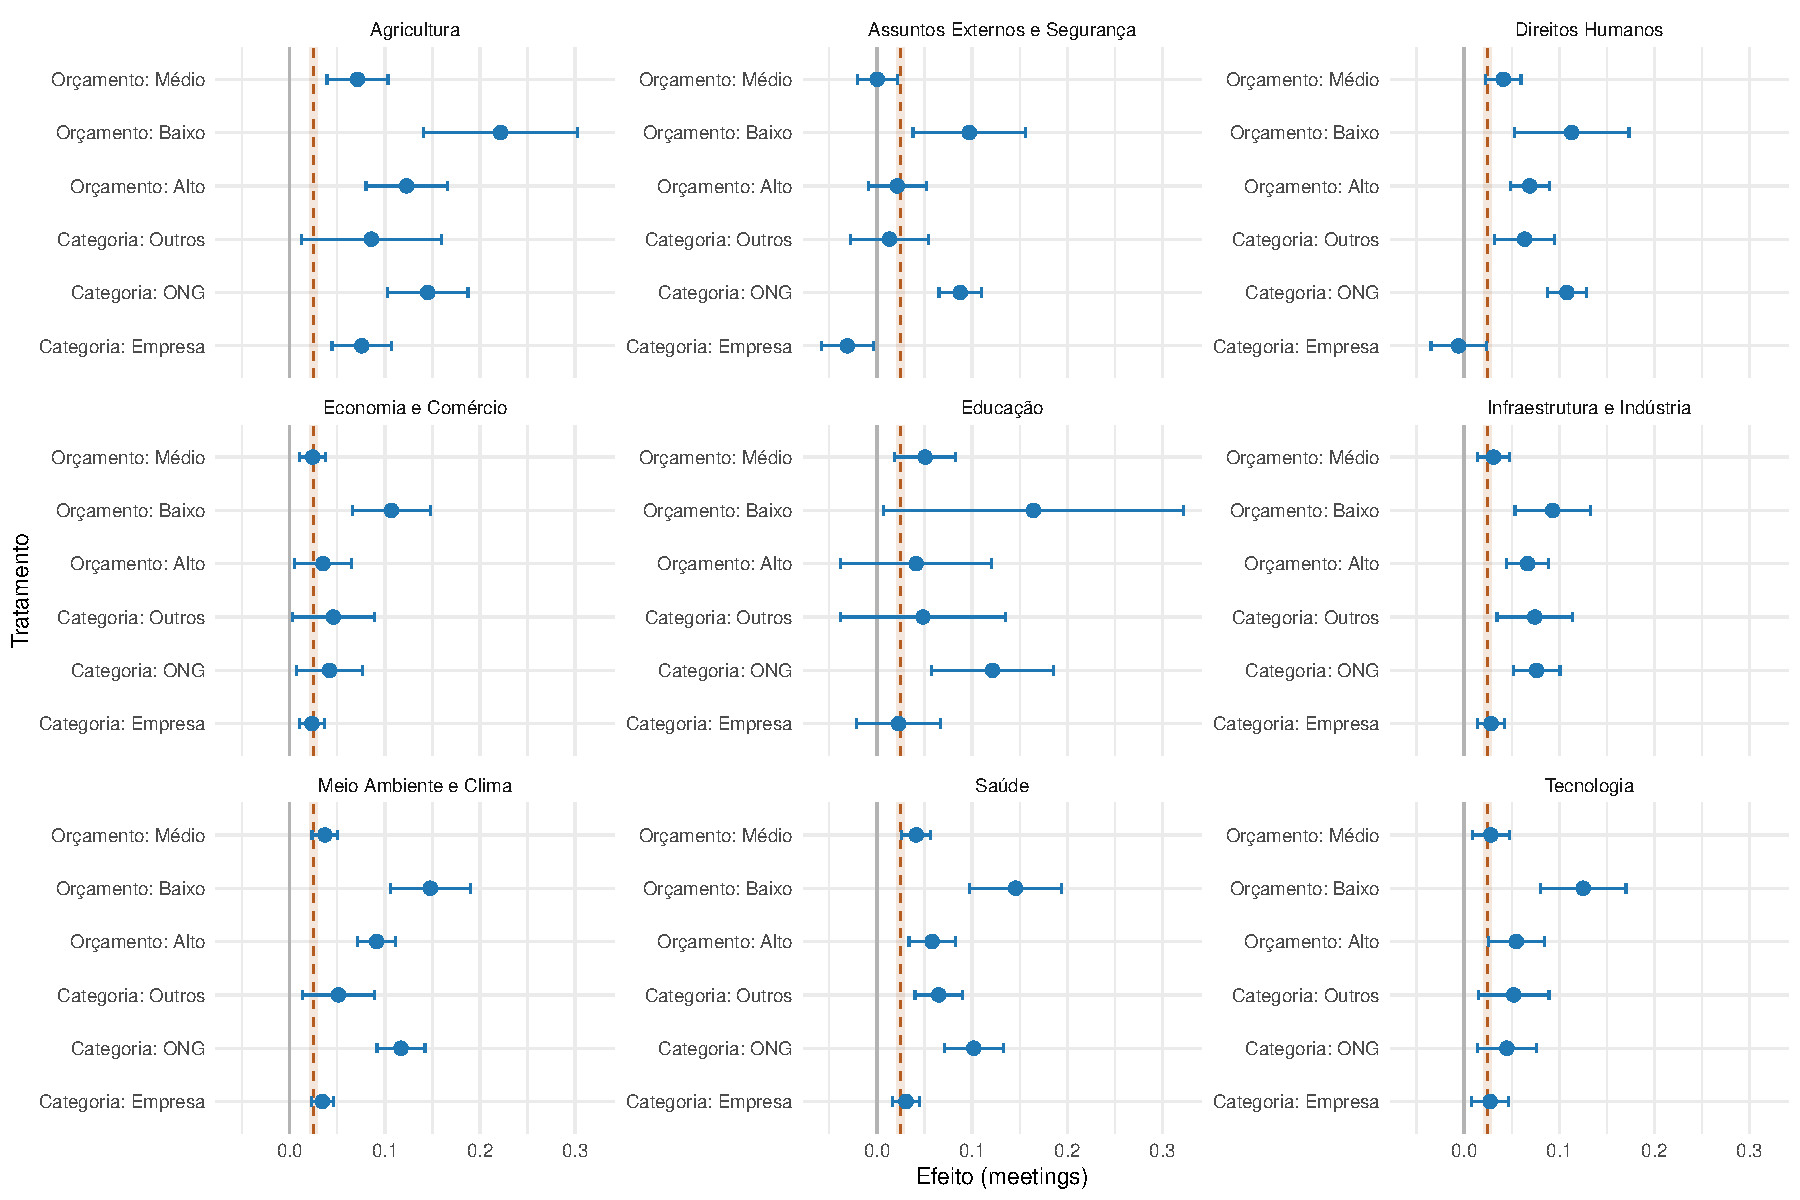
\includegraphics[width=1.2
    \textwidth]{figures/fig_coeff_treatments_by_domain.pdf}
    \caption{Efeito esperado \textit{ceteris paribus}: especificação linear (\acrshort{ppml}) para cada tratamento por domínio} 
    \label{fig:effect_linear_ppml_treatments_by_domain}
\end{figure}
\end{landscape}


